\documentclass[12pt]{article}

\nofiles  % TeX does not produce an *.aux file
\usepackage{color}
\usepackage{graphicx}
\usepackage{fix-cm}
\input{/Users/nychka/Home/Tex/NychkaStuff.tex}
 \input{/Users/nychka/Home/Tex/ColorsFromR.tex}

\setlength{\paperheight}{11in}
\setlength{\paperwidth}{8.5in}
\setlength{\textheight}{8.75in}
\setlength{\textwidth}{6.75in}
\setlength{\evensidemargin}{0.0in}
\setlength{\oddsidemargin}{0.0in}
\setlength{\topmargin}{0in}
\setlength{\parindent}{0in}
\setlength{\parskip}{12pt}
\pagestyle{empty}

  
\begin{document}
\vspace*{-1.5in}
{\sf
{ 
\color{red4}
\hspace*{-.5in} \fontsize{40}{50}\selectfont{ 
Introduction to Data Analysis  \\ with R 
}
}
\\
\\
%\hspace*{-.25in}
\begin{minipage}{7in}{\Large APPM 2720
Mon, Wed, 3 - 4:15 PM, Spring 2016. \\
 Douglas Nychka, 
Affiliate Faculty, Applied Mathematics  \\
\verb+nychka@ucar.edu+
%Scientific Staff, National Center for Atmospheric Research
 }
 \end{minipage}
\\


%\hspace{-.25in}
\begin{minipage}{6.75in}
{\Large
{\it Data science}  is a new field that combines mathematics, computer science, and statistics with the goal of
answering questions and discovering new information from data. 
}
\end{minipage}
%\end{quote}

%

%\hspace{-.25in}
\begin{minipage}{4.5in}
\vspace*{0in}
{\Large
%\begin{itemize}
\bdot How should I buy  a used car on {\tt cars.com}? \\[.125in]
\bdot Where is the steepest part of a ski slope? \\[.125in] 
\bdot How is the climate changing in Colorado? \\[.125in] 
\bdot When will the next flu outbreak occur? \\[.125in] 
\bdot What web pages have similar content?
%\end{itemize}
}
%
\end{minipage}
%
\begin{minipage}{3.in}
\vspace*{0in}
\hspace*{.125in}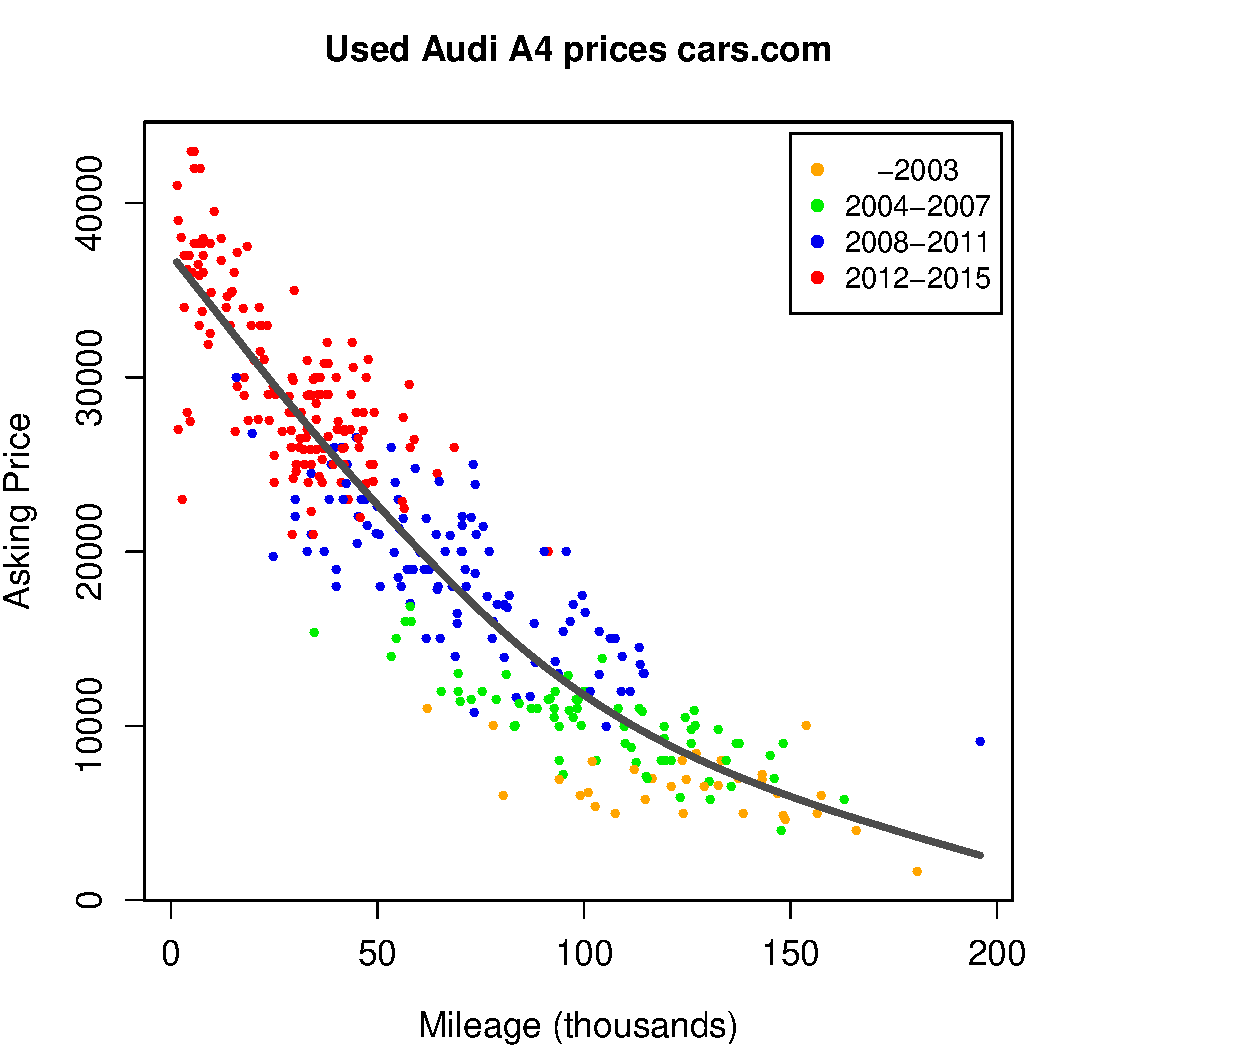
\includegraphics[width=2.5in]{A4.pdf}
\end{minipage}
\\

\hspace*{-.25in}
\begin{minipage}{3in}
\vspace*{0in}
Degree of slope for Riflesight Notch Trail \\
Mary Jane, Colorado  \\
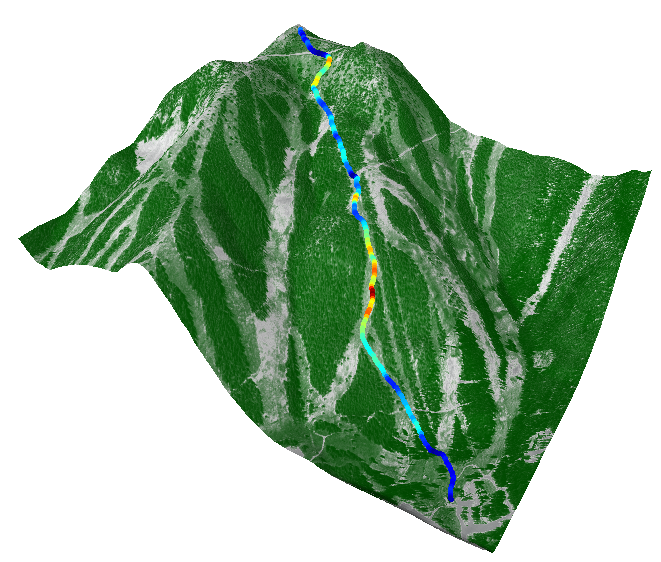
\includegraphics[width=3in]{slopeimage3.png}
\end{minipage}
%
\begin{minipage}{6in}
\vspace*{.25in}
\hspace*{.5in} Daily precipitation amounts  for Boulder \\
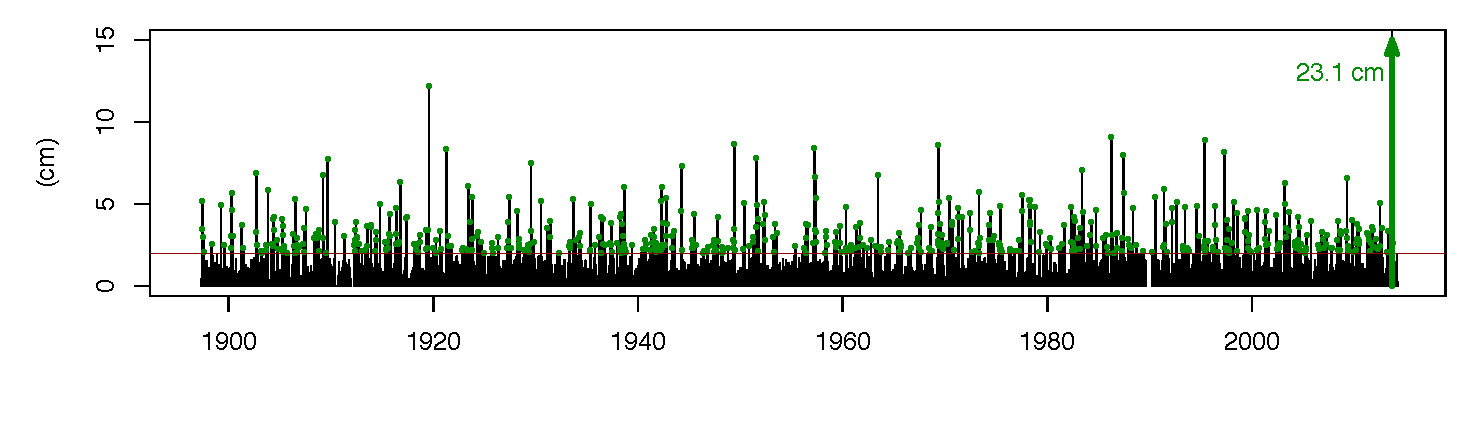
\includegraphics[width=4in, height=2.25in]{/Users/nychka/Home/Current_talks/AGUExtremes/pix/Boulder1.pdf} 
\end{minipage}

%These kind of practical questions require skills in wrangling data sets into forms for analysis, using graphics to explore
%relationships among variables, writing programs to do statistical analysis, 
%and communicating the results in nontechnical language.
{\Large
This course will expose students to practical data analysis and statistics. In the process students will learn how to 
 write programs in the R language and generate figures and reports. 
R is a flexible language similar to Matlab and python, is fun to use, and is
 good for learning how to program. 
 The course will  also introduce students to  modern data analysis tools including 
regression and smoothing, multivariate analysis, clustering, spatial prediction and image analysis.
}
}
\end{document}
